\documentclass{article}
\usepackage{graphicx} % Required for inserting images
\usepackage{amsmath,amssymb, mathtools, dirtytalk}
\graphicspath{{Images/}}

\setlength{\oddsidemargin}{0in}
\setlength{\textwidth}{6.5in}
\setlength{\topmargin}{-.55in}
\setlength{\textheight}{9in}
\pagestyle{empty}


\title{Optimization HW 5}
\author{Michael Nameika}
\date{March 2023}

\begin{document}

\maketitle

\section*{Section 5.4 Problems}
\textbf{1.} Use the simplex method (via a phase-1 problem) to find a basic feasible solution to the following system of linear inequalities:
\begin{align*}
    2x_1 - 3x_2 + 2x_3 &\geq 3\\
    -x_1 + x_2 + x_3 &\geq 5\\
    x_1,x_2,x_3 &\geq 0.
\end{align*}
\newline\newline
See attached work.
\newline\newline
\textbf{2.} Solve the problem
\begin{align*}
    \text{minimize} \:\:\: &z = -4x_1 - 2x_2 - 8x_3\\
    \text{subject to} \:\:\: &2x_1 - x_2 + 3x_3 \leq 30\\
    &x_1 + 2x_2 + 4x_3 = 40\\
    &x_1,x_2,x_3 \geq 0.
\end{align*}
using (a) the two-phase method.
\newline\newline
See attached work.

\section*{Section 6.2 Problems}
\textbf{1.} Consider the linear program 
\begin{align*}
    \text{maximize}\:\:\: &z = -x_1 - x_2\\
    \text{subject to} \:\:\: &-x_1 + x_2 \geq 1\\
    &2x_1 - x_2 \leq 2\\
    &x_1,x_2\geq 0
\end{align*}
Find the dual to the problem. Solve the primal and the dual graphically, and verify that the results of the strong duality theorem hold. Verify that the optimal dual solution satisfies $y^T = c_B^TB^{-1}$ where $B$ is the optimal basis matrix.
\newline\newline
The corresponding dual to this problem is
\begin{align*}
    \text{minimize} \:\:\: &w = y_1 + 2y_2\\
    \text{subject to} \:\: &-y_1 + 2y_2 \geq -1\\
    &y_1 - y_2 \geq -1\\
    &y_1 \geq 0, \: y_2 \leq 0
\end{align*}
Solving the primal problem graphically, as we can see from the figure below, we have that the maximal value is $Z = -1$ at the point $(x_1, x_2)^T = (0,1)$
\begin{center}
    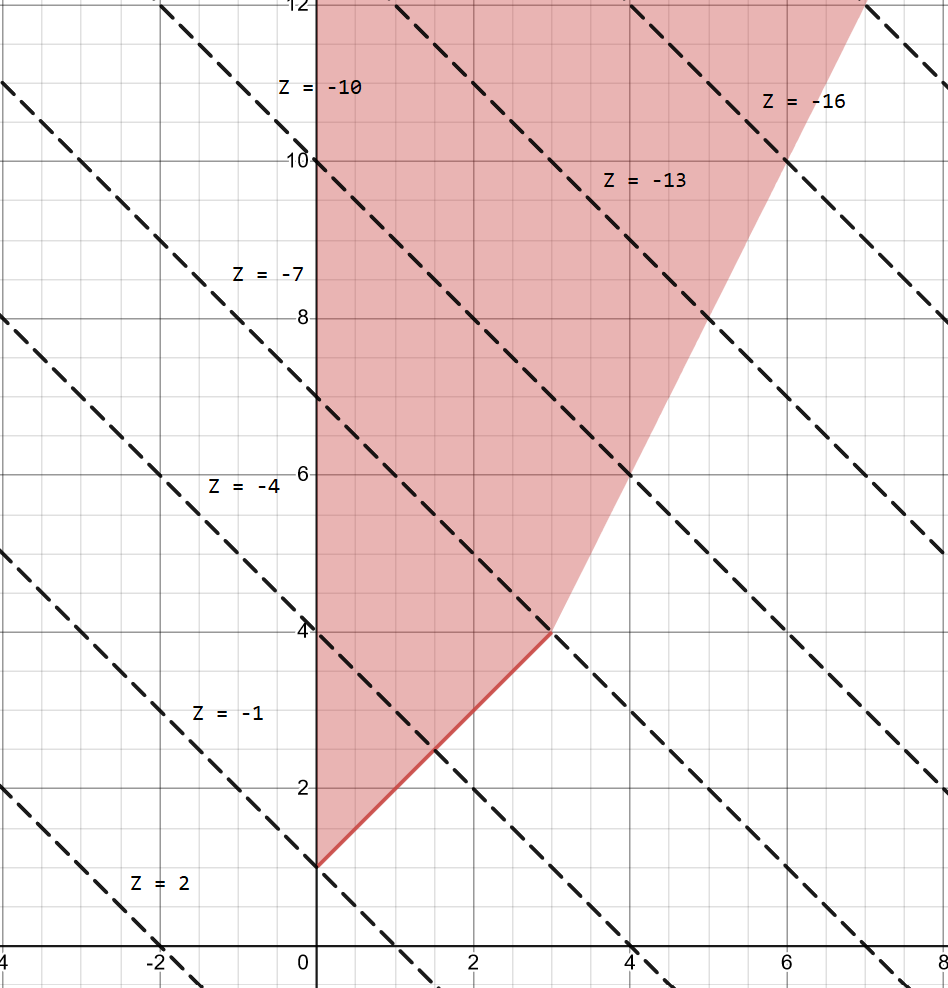
\includegraphics[scale = 0.5]{2.1primal}
\end{center}
Solving the dual problem graphically, we also see from the figure below that the minimal value is $w = -1$ at the point $(y_1,y_2)^T = (0,-1/2)$
\begin{center}
    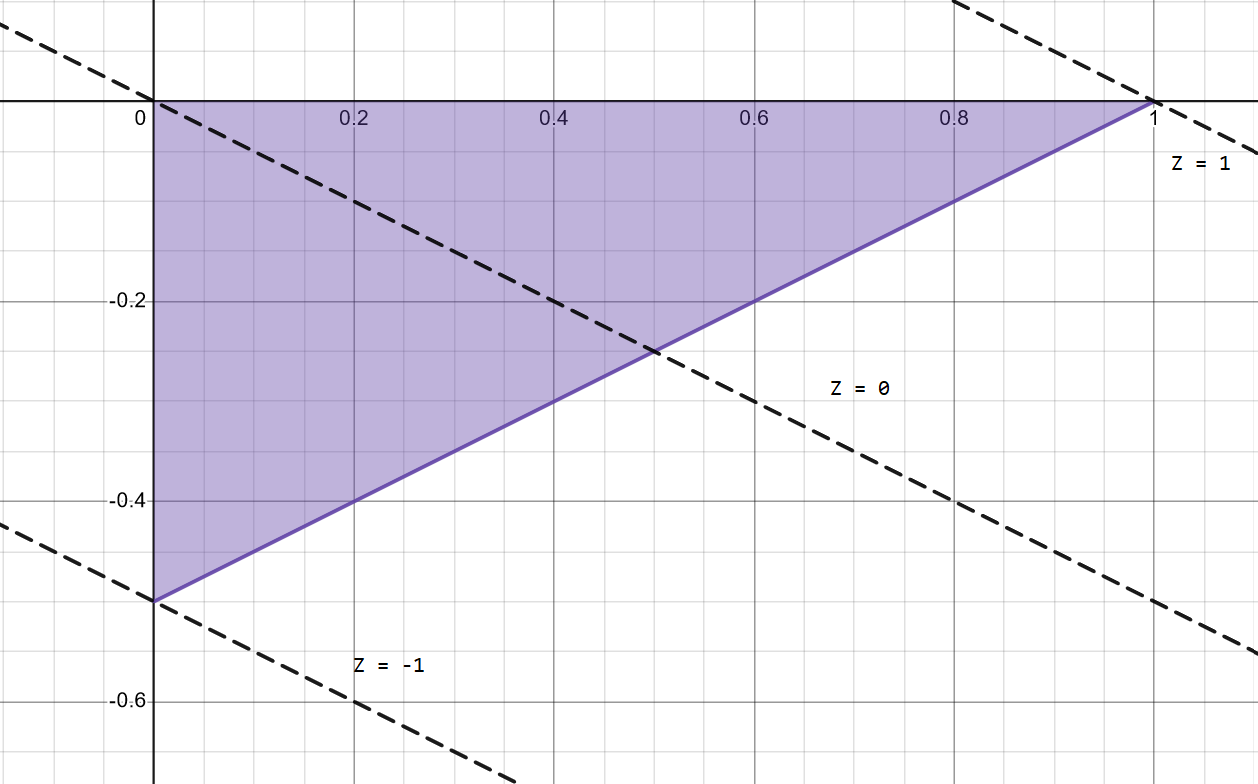
\includegraphics[scale = 0.5]{2.1dual}
\end{center}
Notice that both the primal and the dual have optimal solutions, and those optimal solutions are equal, which agrees with the results of strong duality. Converting the problem to standard form (by introducing an excess variable $x_3$ to the first constraint and the slack variable $x_4$ to the second constraint) and using the simplex method script, we see that the basis $(x_1,x_4)$ is optimal and that $B^{-1} = \begin{pmatrix}
    1 & 0\\
    1 & 1
\end{pmatrix}$, $c_B^T = (1,0)$ and so $c_B^TB^{-1} = (1,0) = y^T$ as we can see in the screenshot below:
\begin{center}
    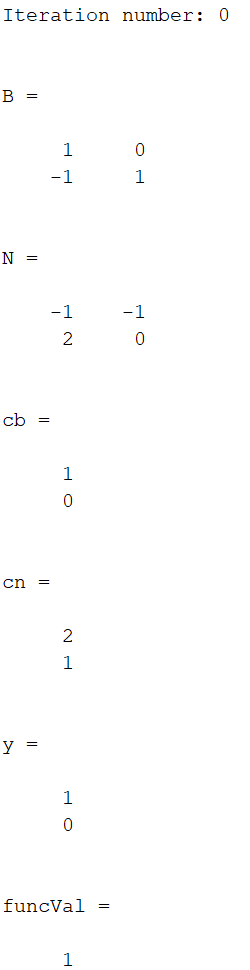
\includegraphics[scale = 0.6]{optimalBasis}
\end{center}
\textbf{3.} Prove Corollary 6.6:
\newline

\textit{If the primal is unbounded, then the dual is infeasible. If the dual is unbounded, then the primal is infeasible.}
\newline\newline
Proof: Consider the primal program written in canonical form:
\begin{align*}
    \text{minimize}\:\:\: &z = c^Tx\\
    \text{subject to} \:\:\: &Ax \geq b\\
    &x \geq 0
\end{align*}
and the corresponding dual:
\begin{align*}
    \text{maximize}\:\:\: &w= b^Ty\\
    \text{subject to} \:\:\: &A^Ty \leq c\\
    &y \geq 0
\end{align*}
And suppose by way of contradiction that the primal is unbounded and that $x$ and $y$ are feasible solutions to the primal and dual, respectively. Then by weak duality, we have 
\[z \geq w\]
That is, $w$ is a lower bound for $z$, but since the primal problem is assumed to be unbounded (and in canonical form), $z$ has no minimal value, a contradiction.
\newline

Now suppose that the dual is unbounded and that $x$ and $y$ are feasible solutions to the primal and dual, respectively. Again by weak duality we have $z \geq w$, so that $z$ is an upper bound for $w$. Since the dual problem is assumed to be unbounded (and in canonical form), $w$ has no maximal value, a contradiction.
\newline\newline\newline
\textbf{4.} Prove Corollary 6.7:
\newline

\textit{If $x$ is a feasible solution to the primal, $y$ is a feasible solution to the dual, and $c^Tx = b^Ty$, then $x$ and $y$ are optimal for their respective problems.}
\newline\newline
Proof: Suppose that $x$ and $y$ are solutions to the the primal and dual, respectively, written in canonical form. Further suppose that $c^Tx = b^Ty$. Recall that the weak duality theorem that $c^Tx \geq b^ty$. That is, $b^ty$ is a lower bound for $c^Tx$, and likewise, $c^Tx$ is an upper bound for $b^Ty$. That is, since we have $c^Tx = b^Ty$, $x$ gives a minimal value for $z$ since any other feasible point $x$ must satisfy $c^Tx \geq b^Ty$. Similarly, $y$ is a maximal value for $w$ by similar logic. That is, $x$ and $y$ are optimal solutions to their respective problems.


\section*{Section 6.4 Problems}
\textbf{1.} The following questions apply to the linear program in Example 6.14. Each of the questions is independent.
\begin{itemize}
    \item[(i)] By how much can the right-hand side of the first constraint change before the current basis ceases to be optimal?
    \newline\newline
    The first constraint in example 16.5 is $-2x_1 + x_2 + x_1 = 2$ in standard form. Recall that the perturbation must satisfy the inequality
    \[B^{-1}b \geq -B^{-1}\Delta b\]
    From the example, we have 
    \[B^{-1} = \begin{pmatrix*}[r]
        0 & 1/2 & -1/2\\
        0 & 0 & 1\\
        1 & 3/2 & 1/2
    \end{pmatrix*}, \:\:\:\:\: \begin{pmatrix*}[r]
        2\\
        7\\
        3
    \end{pmatrix*}\]
    and so $B^{-1}b = (5,3,3)^T$. And since we are perturbing the first constraint, we have $\Delta b = (\delta, 0, 0)^T$ and so $-B^{-1}\Delta b = (0, 0, -\delta)^T$ so we require $(5,3,3)^T \geq (0,0,-\delta)^T$ which gives us $-\delta \leq 3$ or equivalently, $\delta \geq -3$. That is, we can change the right hand side of the first constraint by at least $-3$ to ensure the current basis remains optimal.

    
    \item[(ii)] What would the new solution be if the right-hand side of the third constraint were increased by 5?
    \newline\newline
    Similar to part (i), we have $\Delta b = (0,0,\delta)$, and so our basis will remain feasible only if $B^{-1}b \geq -B^{-1}\Delta b$ and so $(5,3,3)^T \geq (-\delta/2,-\delta,-3/2\delta)^T$. That is, our current basis will remain optimal so long as $\delta \geq -2$, which for this problem, $\delta = 5 > -2$, so our basis remains optimal. Then we have 
    
    \begin{align*}
        \bar{z} &= z + y^T\Delta b\\
        &= -13 + (0,-1,-2)(0,0,5)^T\\
        &= -23
    \end{align*}
    So the new solution is $\bar{z} = -23$.
    \newline\newline
    \item[(iii)] What would the new solution be if the coefficient of $x_1$ in the objective were decreased by 2? Increased by 2?
    \newline\newline
    Let us begin by testing to by how much we can change $c_1$ and our basis remains optimal. Recall that we require
    \[c_N^T - c_B^TB^{-1}N \geq \Delta c_B^TB^{-1}N\]
    For this example, we have $c_B^T = (-2,-1,0)$, $c_N^T = (0,0)$ and $\Delta c_B^T = (0, \delta, 0)$. Then we have 
    \[\Delta c_B^T B^{-1}N = (0,\delta)\]
    and
    \[-c_B^TB^{-1}N = (1,2)\]
    and so we require $(1,2) \geq (0,\delta)$ or $\delta \leq 2$. That is, our basis will remain optimal if we increase or decrease $c_1$ by 2. If we decrease $c_1$ by 2, we have $\Delta c_B^T = (0,-2,0)$ and so
    \begin{align*}
        \bar{z} &= z + \Delta c_B^Tx_B\\
        &= -13 + (0,-2,0)(5,3,3)^T\\
        &= -19
    \end{align*}
    Similarly, if we increase $c_1$ by 2, we get
    \begin{align*}
        \bar{z} &= -13 + (0,2,0)(5,3,3)^T\\
        &= -7
    \end{align*}
    So the new solution would be $-19$ if we decrease $c_1$ by 2 and the solution would be $-7$ if we increase $c_1$ by 2.
\end{itemize}


\end{document}
